\documentclass[12pt]{article}

\usepackage{ktu_thesis_style}
\renewcommand{\sectionbreak}{} % allow sections to flow without forced page breaks

\begin{document}
\raggedbottom
%Title and type
\def\projectTitle{Coffee Leaf Disease Classification Report} 
\def\projectType{Report} 

% Author and reviewers:
\def\projectAuthorName{Gerson David Pinto Chica} 
\def\projectSupervisorNameFirst{Dr. Ar\=unas Lipnickas}
\def\projectSupervisorNameSecond{}
\def\projectReviewerNameFirst{}
\def\projectReviewerNameSecond{}


% Year, city, faculty:
\def\projectYear{2026}
\def\projectCity{Kaunas}
\def\projectFaculty{Faculty of Electrical and Electronics Engineering}
\def\projectStudies{}
\def\projectStudyFieldAndArea{Image Classification and Deep Learning}

\def\projectKeywords{coffee leaf disease; image classification; convolutional neural networks; \
MobileNetV2; transfer learning; plant pathology}



%----------------------------LT---------------------
%------------For Summary/Santrauka page-------------
%---------------------------------------------------
%Title and type
\def\projectTitleLT{Coffee Leaf Disease Classification Report} 
\def\projectTypeLT{Report} 

% Author and reviewers:
\def\projectAuthorNameLT{Gerson David Pinto Chica} 
\def\projectSupervisorNameFirstLT{Dr. Ar\=unas Lipnickas}
\def\projectSupervisorNameSecondLT{}
\def\projectReviewerNameFirstLT{}
\def\projectReviewerNameSecondLT{}


% Year, city, faculty:
\def\projectYearLT{2026}
\def\projectCityLT{Kaunas}
\def\projectFacultyLT{Faculty of Electrical and Electronics Engineering}
\def\projectStudiesLT{}
\def\projectStudyFieldAndAreaLT{Image Classification and Deep Learning}


%Keywords
\def\projectKeywordsLT{coffee leaf disease; image classification; convolutional neural networks; \
MobileNetV2; transfer learning; plant pathology}



\input{TitlePage}


\setcounter{page}{2} % count from title page; print from TOC
\tableofcontents



\clearpage
\listoffigures
\addcontentsline{toc}{section}{\listfigurename} % Adds "List of Figures" to the table of contents

\clearpage
\listoftables
\addcontentsline{toc}{section}{\listtablename} % Adds "List of Tables" to the table of contents

\clearpage
\section*{fNIRS Article}

\textbf{Authors:} Valdas Grigaliunas, Gerson David Pinto Chica, Ramune Kaspere \\
\textbf{Date:} May 2026

\section*{Literature Review Article 1}

This literature analysis concerns functional near-infrared spectroscopy (fNIRS) and machine learning as a medium for predicting neurocognitive and health-related issues. This is achieved by training models on fNIRS data collected from a population sample and by using different machine-learning techniques. The aim is to detect patterns that can be labeled as belonging to certain classes of participants or patients. The development of such models is meant to support clinical tools, provided that the data, labels, and clinical interpretation are properly justified.

Different scientific articles have been analyzed. They cover fNIRS technology, machine-learning classification, deep-learning methods, an fMRI autism study, and MRI segmentation.

\textbf{Keywords:} functional near-infrared spectroscopy; fNIRS; machine learning; deep learning; mental health; neurodevelopmental conditions; cognitive workload; screening; biomarker validation.

\section*{Scope of This Literature Analysis}

This literature analysis considers functional near-infrared spectroscopy and machine-learning algorithms as tools for conducting objective assessments of neurocognitive patterns that may be relevant to mental-health and neurodevelopmental screening. Up to this point, the scientific literature does not justify the stronger claim that fNIRS can diagnose psychiatric disorders. Instead, it supports a more careful hypothesis: fNIRS can track hemodynamic responses during a task, and machine-learning models can learn to differentiate between two or more task states or estimate their characteristics.

Several references cover direct topics related to fNIRS classification and deep learning \cite{Wickramaratne2021,Khan2024,Eastmond2022,Ma2021,Sharmin2025}. Another group of papers relates to neuroimaging classification and automated analysis in adjacent domains, such as functional magnetic resonance imaging and low-field magnetic resonance imaging \cite{Eslami2020,Peiris2024}. Finally, one paper focuses on the role of fNIRS within visual analytics for augmented reality-guided human behavior \cite{Castelo2024}. These papers should not be analyzed as if they all provide the same type of evidence. Some support methodological choices, while others support broader arguments about objective neuroimaging assessment.

\section*{fNIRS Approach}

\subsection*{Wickramaratne and Mahmud \cite{Wickramaratne2021}: fNIRS Task Classification, Not Diagnosis}

Wickramaratne and Mahmud provide an example of how fNIRS time-series data can be represented as images and classified using convolutional neural networks. By using the Gramian Angular Summation Field representation instead of manually selecting temporal or spectral features, their model learns relevant structures from a transformed signal representation. This could be useful if feature-based models are compared with representation-learning approaches in future work.

This paper helps justify the use of image representations or CNNs as one possible modeling direction. However, it should be described as task classification, not disease diagnosis.

\begin{equation*}
\text{Gramian Angular Summation Field representation:}
\end{equation*}

\begin{align*}
\tilde{x}_i &= \frac{x_i - \min(X)}{\max(X) - \min(X)} \\
\varphi_i &= \arccos(\tilde{x}_i) \\
\text{GASF}_{ij} &= \cos(\varphi_i + \varphi_j) \\
\text{GASF}_{ij} &= \tilde{x}_i\tilde{x}_j - \sqrt{1 - \tilde{x}_i^2}\sqrt{1 - \tilde{x}_j^2}
\end{align*}

\textit{Note: These equations explain how the fNIRS time-series signal is transformed into an image representation before being classified by the CNN model.}

\begin{figure}[h]
\centering
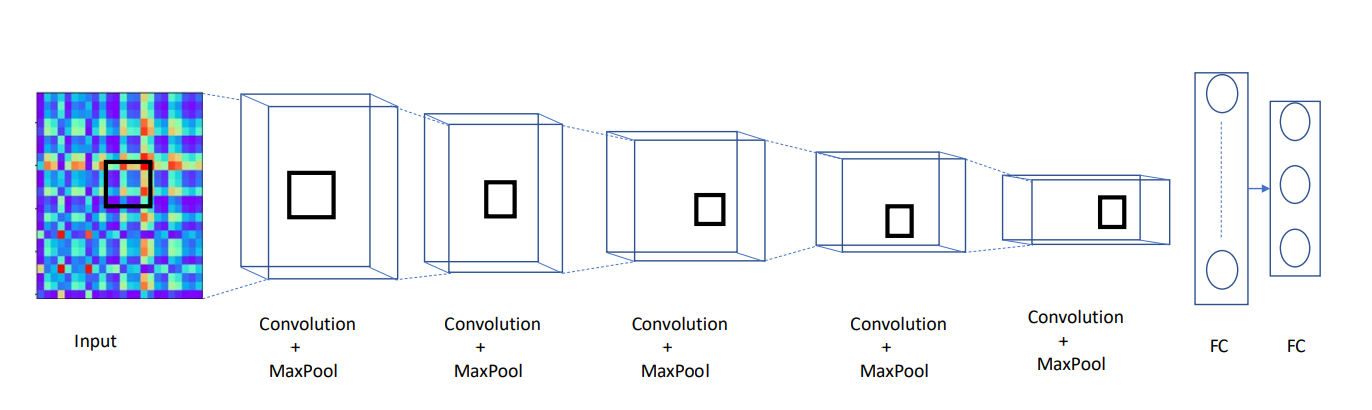
\includegraphics[width=0.8\textwidth]{images/The proposed convolutional networks.png}
\caption{Figure 1. The proposed convolutional neural network used for fNIRS task classification. Source: Wickramaratne and Mahmud [1].}
\label{fig:wickramaratne_fig3}
\end{figure}

\begin{figure}[h]
\centering
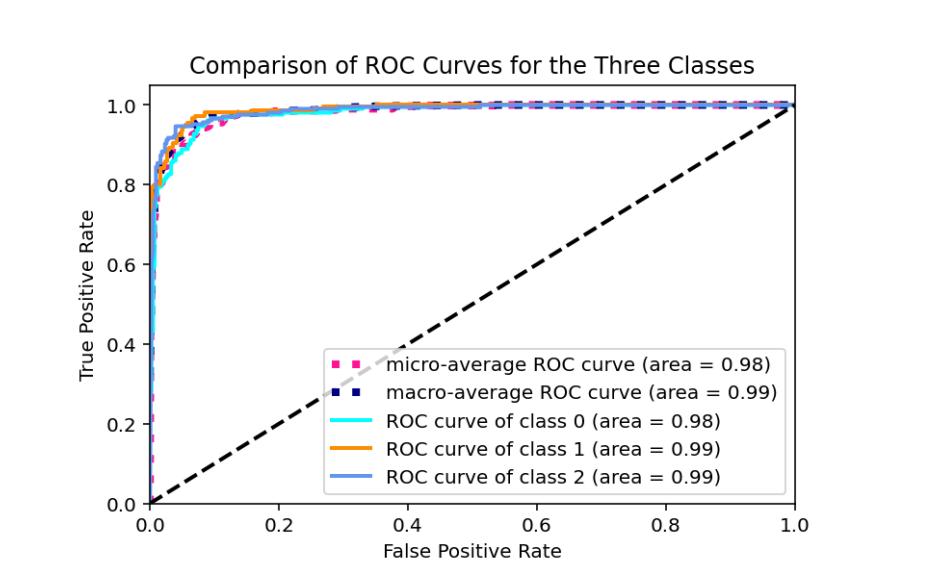
\includegraphics[width=0.8\textwidth]{images/The Comparison for Receiver Operater Characteristic for the three.png}
\caption{Figure 2. Receiver operating characteristic comparison for the three classes using test data from subject 16. Source: Wickramaratne and Mahmud [1].}
\label{fig:wickramaratne_fig4}
\end{figure}

\subsection*{Eslami, Raiker, and Saeed \cite{Eslami2020}}

Eslami, Raiker, and Saeed focus on the application of machine-learning techniques to fMRI and autism spectrum disorder. This is useful because the paper touches on the broader motivation of the thesis: behavioral assessment can be subjective, time-consuming, and difficult to scale, which motivates the search for objective neural biomarkers. However, this paper is not evidence that fNIRS can detect autism. fMRI and fNIRS differ in spatial coverage, cost, equipment mobility, signal characteristics, and experimental design. A result found using fMRI cannot be directly generalized to fNIRS without further studies.

\subsection*{Castelo et al. \cite{Castelo2024}: Ecological Assessment and Multimodal Behavior}

Castelo et al.\ use fNIRS in the field of human behavior assessment through visual analytics and augmented reality assistance. The paper does not focus on clinical problems; nevertheless, it is useful because it shows that fNIRS can be used outside purely laboratory-based studies. It supports the idea that fNIRS can contribute to ecological and multimodal assessment, especially when combined with other sensor streams such as gaze and motion data.

\subsection*{Peiris and Chen \cite{Peiris2024}: Deep Learning-Based Automated Neuroimaging Analysis}

Peiris and Chen describe the use of deep learning for the segmentation of bilateral hippocampi using low-field MRI. At first, this paper may not seem directly relevant to fNIRS. Indeed, it does not contribute to fNIRS signal classification, hemodynamic task analysis, or mental-health prediction based on wearable optical measurements. Its relevance is indirect. The motivation behind low-field MRI and fNIRS is partly related to accessibility: researchers and clinicians need tools that are cheaper, easier, and faster than expensive MRI or PET scanners. However, accessibility alone is not enough; the method must measure the correct variable and be valid for its intended purpose.

This reference should be kept only if the literature review includes a short comparison with adjacent neuroimaging methods. Otherwise, it can be removed to keep the review more focused.

\subsection*{Khan et al. \cite{Khan2024}: CNN + LSTM Neural Network Model for fNIRS Workload Classification}

Khan et al.\ provide one of the most relevant methodological references. Their proposed deep-learning architecture is consistent with the characteristics of fNIRS data. The signal is multidimensional because it varies across multiple channels and changes over time. Therefore, a CNN model can identify spatial dependencies between channel values, while an LSTM can account for temporal dependencies.

Workload classification is different from disease diagnosis. Classification means that the algorithm distinguishes between different experimental conditions, and those conditions may reflect task complexity, cognitive load, effort, arousal, time constraints, or other factors. However, this does not necessarily indicate disorder-specific physiology.

\begin{figure}[h]
\centering
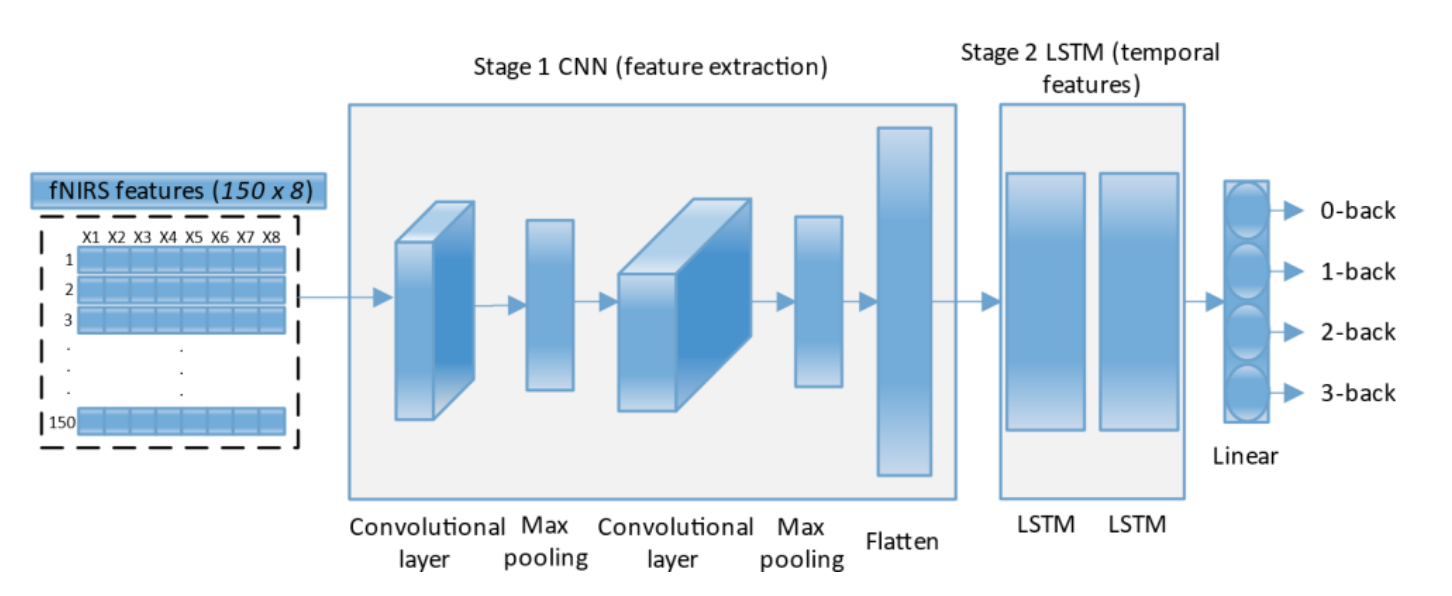
\includegraphics[width=0.8\textwidth]{images/The diagram illustrates the proposed architecture, incorporating both CNN and LSTM.png}
\caption{Figure 3. Proposed architecture incorporating CNN and LSTM layers for fNIRS workload classification. Source: Khan et al. [5].}
\label{fig:khan_fig1}
\end{figure}

\begin{equation*}
\text{Convolution operation and related functions:}
\end{equation*}

\begin{align*}
Y[i] &= f\left(\sum_{j=1}^{k} X[i + j - 1] \cdot W[j] + b\right) \\
Y[i] &= \max(0, X[i]) \quad \text{(ReLU activation)} \\
Y[i] &= \max(X[i \cdot p : (i+1) \cdot p]) \quad \text{(Max-pooling operation)}
\end{align*}

\begin{equation*}
\text{LSTM equations:}
\end{equation*}

\begin{align*}
i_t &= \sigma(U_i * X_t + V_i * H_{t-1} + Z_i \circ C_{t-1} + b_i) \quad \text{(Input gate)} \\
f_t &= \sigma(U_f * X_t + V_f * H_{t-1} + Z_f \circ C_{t-1} + b_f) \quad \text{(Forget gate)} \\
o_t &= \sigma(U_o * X_t + V_o * H_{t-1} + Z_o \circ C_{t-1} + b_o) \quad \text{(Output gate)} \\
\tilde{C}_t &= \tanh(U_c * X_t + V_c * H_{t-1} + b_c) \quad \text{(Candidate cell state)} \\
C_t &= f_t \circ C_{t-1} + i_t \circ \tilde{C}_t \quad \text{(Cell state)} \\
H_t &= o_t * \tanh(C_t) \quad \text{(Hidden state)}
\end{align*}

\textit{Note: The CNN part extracts spatial/local features from fNIRS signals, while the LSTM part models temporal dependencies in the signal.}

\subsection*{Eastmond et al. \cite{Eastmond2022}}

Eastmond et al.\ provide a useful review for justifying the inclusion of deep-learning models in an fNIRS literature review. The paper also helps explain the methodological risks of applying deep learning to fNIRS data. These risks include small sample sizes, noisy labels, motion artifacts, overfitting, and limited clinical interpretation. Complex models may achieve high accuracy while learning shortcuts instead of physiologically meaningful patterns.

This reference is important because it supports a cautious interpretation of deep-learning performance. It also supports the need to compare deep models with simpler baseline models and to clearly report validation methods.

\begin{figure}[h]
\centering
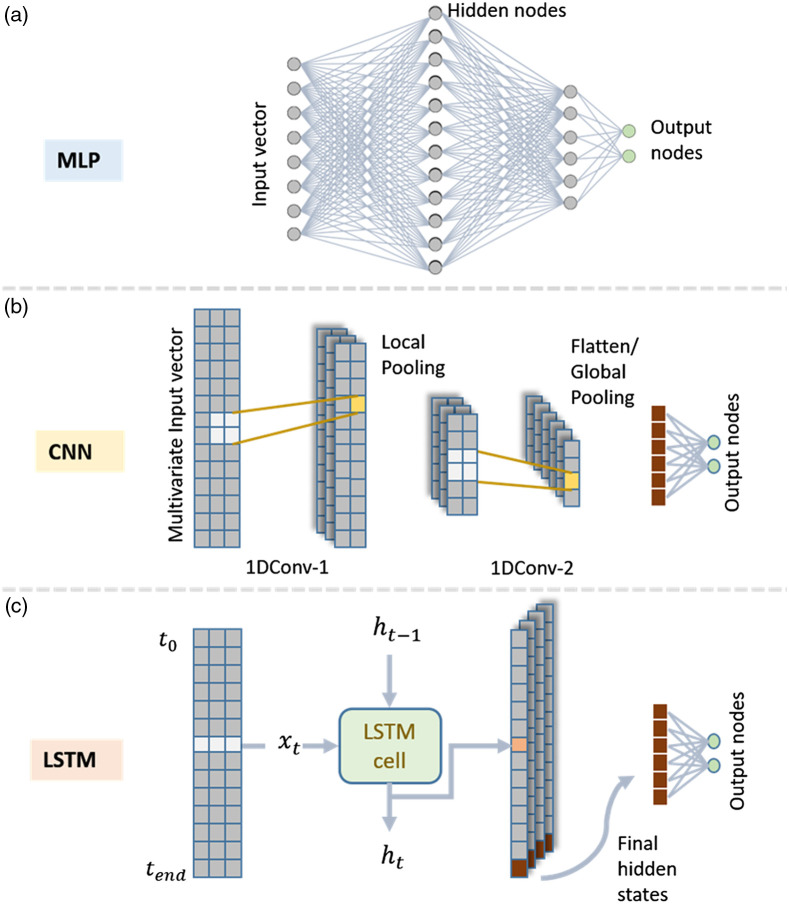
\includegraphics[width=0.8\textwidth]{images/shows MLP, CNN, and LSTM architectures..jpg}
\caption{Figure 4. Common deep-learning architectures used in fNIRS studies: MLP, CNN, and LSTM. Source: Eastmond et al. [6].}
\label{fig:eastmond_fig1}
\end{figure}

\begin{figure}[h]
\centering
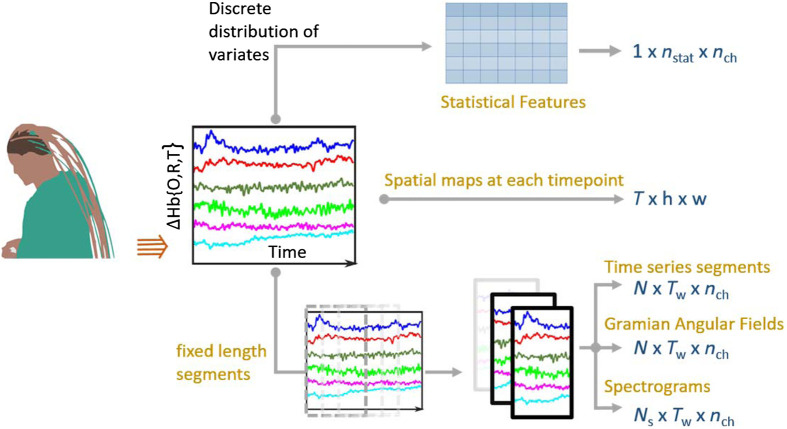
\includegraphics[width=0.8\textwidth]{images/extraction of samples for training neural networks..jpg}
\caption{Figure 5. Extraction of samples for training neural networks from fNIRS data. Source: Eastmond et al. [6].}
\label{fig:eastmond_fig2}
\end{figure}

\begin{equation*}
\text{Activation functions and loss functions:}
\end{equation*}

\begin{align*}
\sigma(x) &= \frac{1}{1 + e^{-x}} \quad \text{(Sigmoid activation)} \\
\text{softmax}(z_i) &= \frac{e^{z_i}}{\sum_j e^{z_j}} \quad \text{(Softmax activation)} \\
\text{ReLU}(x) &= \max(0, x) \quad \text{(ReLU activation)} \\
L &= -\sum_i y_i \log(\hat{y}_i) \quad \text{(Cross-entropy loss)} \\
\text{MSE} &= \frac{1}{n}\sum_i(y_i - \hat{y}_i)^2 \quad \text{(Mean squared error)}
\end{align*}

\textit{Note: These equations explain basic neural-network functions and losses commonly used in deep-learning models for fNIRS classification.}

\subsection*{Ma et al. \cite{Ma2021}: Walking-Task Classification in Older Adults}

Ma et al.\ classify walking task states in older adults using fNIRS. This is a relevant population because older adults may experience functional or cognitive decline. In addition, dual-task walking can reflect higher cognitive and motor demands. This makes the study closer to a real health-assessment context than a purely artificial laboratory task.

However, the labels are still experimental task states rather than direct clinical diagnoses. Therefore, this paper can support the idea that fNIRS is useful for functional assessment, but it should not be presented as proof that fNIRS can diagnose a disorder.

\begin{figure}[h]
\centering
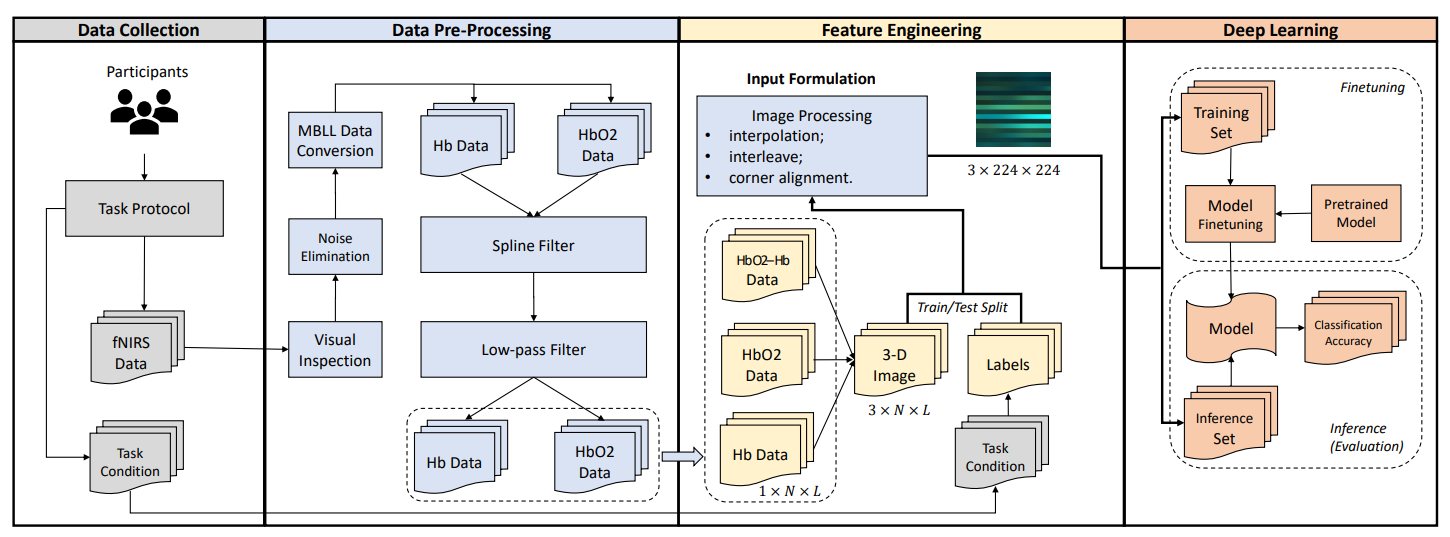
\includegraphics[width=0.8\textwidth]{images/proposed framework for walking-task classification using fNIRS..png}
\caption{Figure 6. Proposed framework for walking-task classification using fNIRS data. Source: Ma et al. [7].}
\label{fig:ma_fig1}
\end{figure}

\begin{figure}[h]
\centering
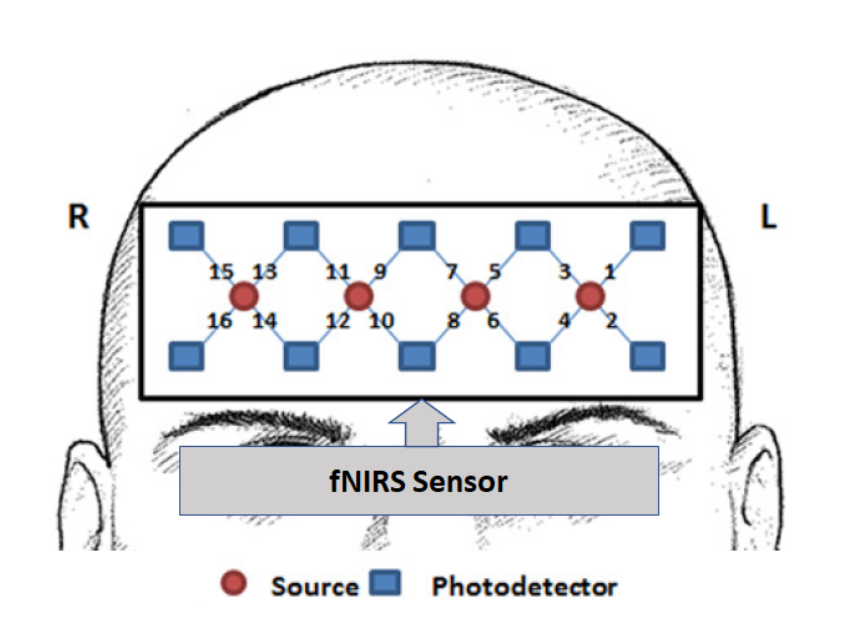
\includegraphics[width=0.8\textwidth]{images/fNIRS sensor pad and forehead voxel locations.png}
\caption{Figure 7. fNIRS sensor pad and forehead voxel locations used for data acquisition. Source: Ma et al. [7].}
\label{fig:ma_fig2}
\end{figure}

\begin{equation*}
\text{fNIRS data representation for classification:}
\end{equation*}

\begin{align*}
\text{OI} &= \text{HbO}_2 - \text{Hb} \quad \text{(Oxygenation index)} \\
\text{Input}_i &= 3 \times N_i \times L_i \quad \text{(Input image tensor)} \\
N_i &\leq 16 \quad \text{(Number of voxel locations)} \\
L_i &= 2 \times T_i \quad \text{(Signal length representation)} \\
\text{Input} &= 3 \times 224 \times 224 \quad \text{(Final resized image input)}
\end{align*}

\textit{Note: These equations show how Ma et al.\ formulate fNIRS data as a 3-channel image input for deep-learning-based walking-task classification.}

\subsection*{Sharmin et al. \cite{Sharmin2025}: Cognitive Effort as a Better Bridge than Diagnosis}

Sharmin and colleagues' paper is important because it focuses on cognitive effort rather than only task categories. This is useful for the thesis because cognitive effort may provide a more careful bridge between fNIRS signals and mental-health-related assessment. A person may complete a task successfully but require a high amount of cognitive effort to do so. This difference may be relevant for understanding cognitive strain, fatigue, workload, or mental-health-related functioning.

\begin{figure}[h]
\centering
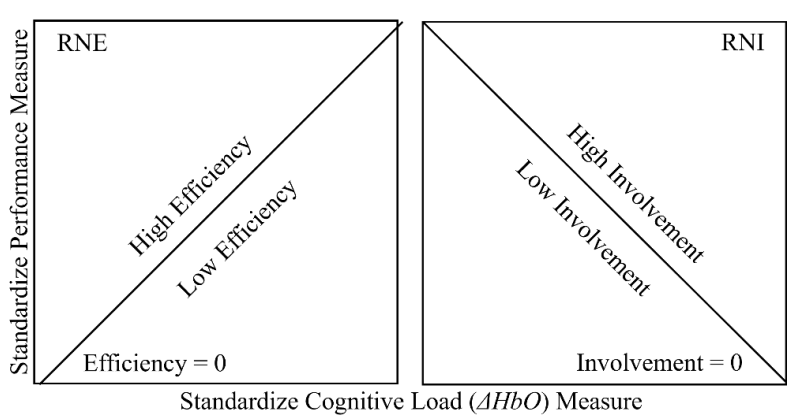
\includegraphics[width=0.8\textwidth]{images/onceptual plots illustrating Relative Neural Efficiency and Relative Neural Involvement.png}
\caption{Figure 8. Conceptual plots illustrating Relative Neural Efficiency and Relative Neural Involvement. Source: Sharmin et al. [8].}
\label{fig:sharmin_fig1}
\end{figure}

\begin{figure}[h]
\centering
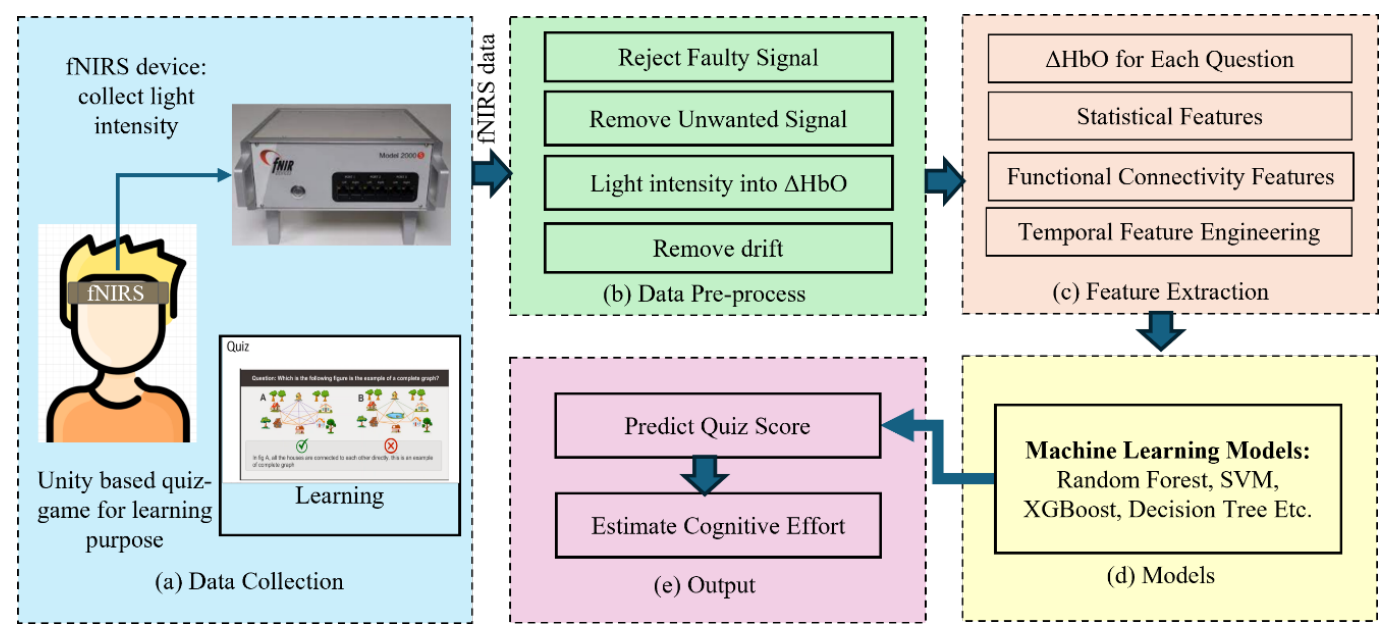
\includegraphics[width=0.8\textwidth]{images/overview of the machine-learning pipeline.png}
\caption{Figure 9. Overview of the machine-learning pipeline for estimating cognitive effort from fNIRS data. Source: Sharmin et al. [8].}
\label{fig:sharmin_fig4}
\end{figure}

\begin{figure}[h]
\centering
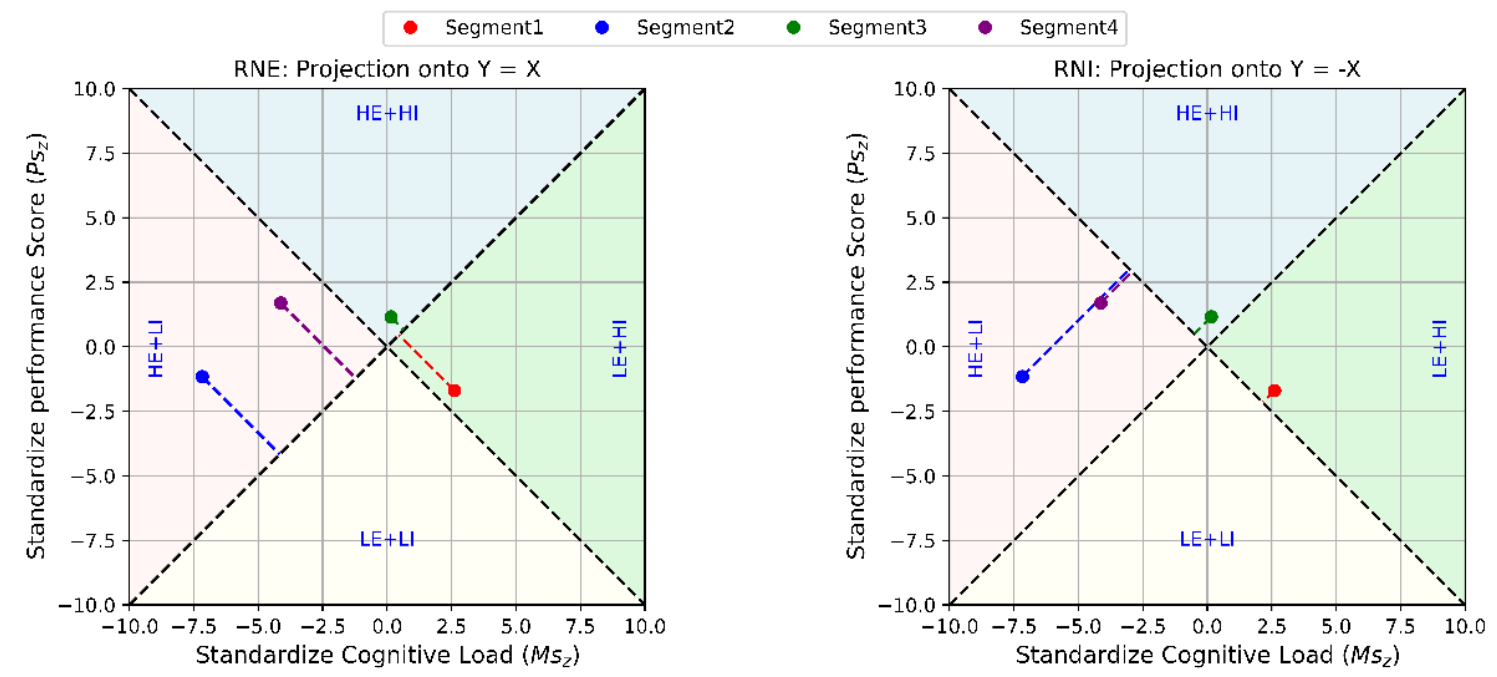
\includegraphics[width=0.8\textwidth]{images/standardized cognitive load and standardized performance across four quiz sessions.png}
\caption{Figure 10. Standardized cognitive load and standardized performance used to represent cognitive-effort states. Source: Sharmin et al. [8].}
\label{fig:sharmin_fig5}
\end{figure}

\begin{equation*}
\text{Cognitive effort framework and evaluation metrics:}
\end{equation*}

\begin{align*}
z &= \frac{x - \mu}{\sigma} \quad \text{(Z-score standardization)} \\
P_z(s, i) &= \frac{P(s, i) - \mu(P_i)}{\sigma(P_i)} \quad \text{(Participant-specific standardized performance)} \\
M_z(s, i) &= \frac{M(s, i) - \mu(M_i)}{\sigma(M_i)} \quad \text{(Participant-specific standardized cognitive load)} \\
\text{RNE} &= \frac{P_z - M_z}{\sqrt{2}} \quad \text{(Relative Neural Efficiency)} \\
\text{RNI} &= \frac{P_z + M_z}{\sqrt{2}} \quad \text{(Relative Neural Involvement)} \\
\text{MAE} &= \frac{1}{n}\sum_i |y_i - \hat{y}_i| \quad \text{(Mean absolute error)} \\
r &= \frac{\sum_i(x_i - \bar{x})(y_i - \bar{y})}{\sqrt{\sum_i(x_i - \bar{x})^2 \sum_i(y_i - \bar{y})^2}} \quad \text{(Pearson correlation)}
\end{align*}

\textit{Note: These equations connect behavioral performance and fNIRS-derived physiological response into one interpretable cognitive-effort framework. MAE and Pearson correlation can be used to compare actual and predicted cognitive-effort values.}

\section*{Cross-Study Interpretation}

Overall, the reviewed sources support the methodological feasibility of studying task states using fNIRS more strongly than they support diagnostic applications for mental-health assessment. Specifically, the literature supports the possibility of classifying task states, workloads, walking conditions, and cognitive-effort patterns from fNIRS data under controlled experimental conditions \cite{Wickramaratne2021,Khan2024,Eastmond2022,Ma2021,Sharmin2025}.

There has been significant progress in classifying fNIRS signals. However, more work is needed before such methods can be used for clinical screening. This requires suitable datasets, clinically meaningful labels, participant-wise validation, external testing, and careful interpretation of model outputs.

\section*{Methodological Implications}

Traditional machine-learning models, such as logistic regression, support vector machines, random forests, and linear discriminant analysis, should remain baseline models for comparison. If a CNN, LSTM, or CNN+LSTM model performs better than simpler models, this improvement should be clearly compared against the baseline results. Otherwise, it is difficult to prove that the more complex model adds scientific or practical value.

The data-splitting scheme is very important. Randomly splitting time windows without considering which participant they came from may lead to an overoptimistic result. In that case, the model may learn participant-specific physiology or artifacts instead of generalizable task-related patterns. Participant-wise splitting is strongly recommended, especially if the thesis aims to make claims about generalization. At minimum, the splitting method should be stated clearly and unambiguously.

Model interpretability is also important. If the outcome variable is related to mental health, neurocognitive state, or a neuropsychiatric condition, the thesis should explain which channels, time windows, or features contributed to the prediction. Feature-importance measures, ablation studies, channel-importance analysis, or comparisons of HbO and HbR responses would increase the scientific value of the work.

\section*{Summary of Key References}

\cite{Wickramaratne2021}, \cite{Khan2024}, \cite{Eastmond2022}, \cite{Ma2021}, and \cite{Sharmin2025} demonstrate that fNIRS combined with machine learning can classify task states and estimate cognitive effort, but the path from task classification to clinical mental-health screening requires careful validation, appropriate datasets, and transparent reporting of limitations.

\par
\section{Conclusion}

This report compared two image-classification approaches for coffee leaf disease
recognition on the same dataset and evaluation split. The Simple CNN achieved the best
test performance in this run, with 95.88\% accuracy, while MobileNetV2 reached 94.43\%.

The results also show that model quality should be interpreted together with efficiency.
MobileNetV2 trained much faster in the frozen-base setting, which is important for rapid
iterations and practical deployment constraints.

The main takeaway is not that one model is universally superior, but that each approach
offers different advantages. Simple CNN provided stronger test metrics in this run,
whereas MobileNetV2 provided better training efficiency. For final submission quality,
future experiments should correct MobileNetV2 preprocessing, evaluate the fine-tuned
stage explicitly, and strengthen data-splitting controls against leakage.




\clearpage 
\phantomsection 
\addcontentsline{toc}{section}{References}
\bibliography{dummy-bib} % And adding references itself

% To know how many pages
\clearpage
\label{LastPage}
\end{document}
